\appendix 
\addcontentsline{toc}{chapter}{Appendix}

\addtocontents{toc}{\protect\setcounter{tocdepth}{-1}}

\chapter{Reflexion - Saif Al-Dilaimi}
\textbf{Hat sich die Aufgabenstellung oder Ihr Verständnis der Aufgabenstellung im Laufe
der Zeit verändert? Wenn ja, wie?}

Das Ergebnis der Anwendung war klar definiert, das Verständnis und das resultierende
Vorgehen zur Bewältigung der Aufgabe war nach dem Erstellen des Pflichtenheftes definiert.
Zunächst war es notwendig sich in den Format der HumanDO.obo Datei einzuarbeiten. Daraufhin wurden alle Arbeitspakete nach Zeitplan absolviert.
\\

\textbf{Wie passend war die Planung des Projektverlaufs, insbesondere der Termine? Wie
häufig musste die Planung angepasst werden? Warum? Was war Ihre Rolle dabei?}

Die Planung und Aufgabenteilung wurde bereits früh im Pflichtenheft festgelegt. Dadurch konnten alle Teammitglieder selbstständig die einzelnen Arbeitspakete durchführen. Mit unserem Betreuer wurden 1-2 mal im Monat Besprechungen eingeplant und aktuelle Themen diskutiert. Als Teamleiter war ich für die Abstimmung verschiedener Aspekte des Projekts zuständig.
\\

\textbf{Welche Methoden haben Sie zur Unterstützung der gemeinsamen Planung genutzt
und wie haben sie sich bewährt?}

Zur gemeinsamen Planung haben wir online Medien genutzt. Über Github konnten wir die kollaborative Zusammenarbeit am Quellcode durchführen. Des Weiteren haben wir auch darüber die Reviews der einzelnen Komponenten durchgeführt. Für die bessere Planung wurden unter anderem Arbeitspakete und Meilensteine im Pflichtenheft erstellt.
\\

\textbf{Wie hat die Koordination bei der Projektarbeit funktioniert? Welche Probleme gab
es? Wie wurden sie angegangen? Was war Ihre Rolle dabei?}

Die Koordination bei der Projektarbeit ging anhand von wöchentlich gesetzten Zielen und
deren Aufteilung problemlos vorwärts. Durch Github und persönlichen Austausch konnten alle Komponenten reibungslos zusammengeführt werden.
\\

\textbf{In wieweit waren Sie ausreichend kompetent für die Mitarbeit? Welche Kompetenzen
mussten Sie sich im Projektverlauf aneignen? Was haben Sie durch das
Studienprojekt gelernt?}

Aufgrund der Größe des Softwareprojektes war es notwendig, auf strukturierte Planung und
Aufgabenteilung innerhalb des Teams zurückzugreifen. Erlernt und vertieft wurde vor allem die Sensibilität und Notwendigkeit von Planung und die Anwendung von Design-Patterns. Insbesondere wurde hier das theoretische Wissen über das Gebiet der Bioinformatik vertieft.
\\

\textbf{Was haben Sie unternommen, um möglichst effizient und verlässlich im Projekt
mitzuarbeiten?}

Für die effiziente und verlässliche Umsetzung wurde auf strukturierte Planung der
einzelnen Programmablaufschritte und zielgerichtete Absprachen unter den
Projektmitgliedern zurückgegriffen. Es war wichtig offene Fragen so früh wie möglich zu
identifizieren und mit den Projektleitern zu besprechen. Die, zu jeder Projektzeit, aktuelle
technische Dokumentation ermöglichte es, den Programmcode einfach, erweiterbar und
wartbar zu halten.
\\

\textbf{Was würden Sie anders machen, wenn Sie mit der zum Projektende erworbenen
Erfahrung die Aufgabe nochmals bearbeiten müssten?}

Da bereits früh das Pflichtenheft erstellt wurde und die Anforderungen definiert wurden, besteht nicht der Wunsch es anders zu wiederholen.
\\

\textbf{Welche Herausforderungen ergaben sich hinsichtlich der Gruppendynamik im Team
und wie sind Sie damit umgegangen?}

In der Durchführung eines Projekts ist die Kommunikation sehr wichtig. Aus diesem Grund haben wir bereits bei der Verkündung der Projektmitglieder zueinander Kontakt aufgenommen und eine Whatsapp-Gruppe gegründet für eine bessere Kommunikation. Daher sah ich keine Herausforderung in diesem Aspekt.
\newpage
\chapter{Reflexion - Dejan Babic}

Die Aufgabenstellung wurde an den ersten Treffen mit unserem Studienprojektbetreuer festgelegt. Um das Projekt grob planen zu können haben wir ein Pflichtenheft erstellt, in welchem die wichtigsten Projektschritte aufgeführt wurden.
\\

\textbf{Wie passend war die Planung des Projektverlaufs, insbesondere der Termine? Wie
häufig musste die Planung angepasst werden? Warum? Was war Ihre Rolle dabei?}

Dadurch, dass wir uns schon relativ früh Gedanken gemacht haben wie das Projekt ablaufen soll haben wir uns dafür entschieden ein Pflichtenheft zu erstellen. Die Erstellung des Pflichtenhefts war zu Anfang des Projekts ein wichtiger Teil, welcher auch von unserem Betreuer abgesegnet wurde.
\\

\textbf{Welche Methoden haben Sie zur Unterstützung der gemeinsamen Planung genutzt
und wie haben sie sich bewährt?}

Zu Beginn des Projekts haben wir festgelegt, dass wir uns die meiste Zeit über Whatsapp oder Teamspeak(Sprachchat) unterhalten werden. Zudem kamen auch einige Treffen in der Uni hinzu.
\\

\textbf{Wie hat die Koordination bei der Projektarbeit funktioniert? Welche Probleme gab
es? Wie wurden sie angegangen? Was war Ihre Rolle dabei?}

Die Koordination war sehr gut. Durch das frühe Beginnen wollten wir verhindern, dass wir in Zeitdruck geraten. Das Pflichtenheft war dabei eine sehr große Hilfe. Probleme gab es eigentlich keine. Das größte Problem war es gemeinsame Termine zu finden um sich miteinander zu treffen.
\\

\textbf{In wieweit waren Sie ausreichend kompetent für die Mitarbeit? Welche Kompetenzen mussten Sie sich im Projektverlauf aneignen? Was haben Sie durch das Studienprojekt gelernt?}

Es ist das zweite mal, dass ich an so einem großen Projekt mitgewirkt habe. Durch das erste Studienprojekt im Bachelorstudium wusste ich wie ein Projekt dieser Größe abläuft und konnte vieles aus dem ersten Studienprojekt nun im zweiten wiederverwenden. Vor Allem die Planung lief dieses mal noch koordinierter ab.
Durch das Projekt habe ich erstmals einen praktischen Bezug zu Datenbanken gemacht. Jedoch konnte ich mich mithilfe der grundlegenden Kenntnisse aus der Bachelorvorlesung Datenbanksysteme sehr gut in die Thematik einarbeiten. 
Das Projekt war eine gute praxisbezogene Arbeit, bei welcher ich weitere Erfahrung gesammelt habe im Team zu arbeiten.
\\

\textbf {Was haben Sie unternommen, um möglichst effizient und verlässlich im Projekt mitzuarbeiten?}

Nach der Erstellung des Pflichtenhefts wurden die Aufgabenteile an die verschiedenen Gruppenmitglieder verteilt und es wurde angefangen zu arbeiten. Ich habe versucht meinen Teil des Projekts so gut es geht zu bearbeiten. Als Ziel habe ich mir gesetzt früher als gewollt fertig zu werden. Wenn Probleme oder Unklarheiten gab habe ich so schnell wie möglich nach Problemlösungen zu suchen oder meine Teammitglieder um Rat gebeten.
\\

\textbf {Was würden Sie anders machen, wenn Sie mit der zum Projektende erworbenen Erfahrung die Aufgabe nochmals bearbeiten müssten?}

Dadurch, dass alle Teammitglieder schon einmal ein Projekt bearbeitet hatten, legten wir von Anfang an eine sehr geordnete und koordinierte Vorgehensweise an den Tag. Die Erstellung des Pflichtenhefts zu Anfang hat enorm viel zum Verständnis der Planung des Projekts beigetragen.
\\

\textbf {Welche Herausforderungen ergaben sich hin sichtlich der Gruppendynamik im Team und wie sind Sie damit umgegangen?}

Das größte Problem waren unsere unterschiedlichen Stundenpläne.
Dadurch, dass wir uns recht früh am Anfang des Projektes schon Gedanken darüber gemacht haben wann wir uns für das Studienprojekt treffen wollen, waren immer schnell passende Termine gefunden. 
Diese frühe Planung hat uns enorm geholfen keinen Zeitdruck zu bekommen. Zudem haben wir uns bei Problemen immer über Whatsapp oder Mail erreichen können.

\newpage
\chapter{Reflexion - Arlind Avdullahu}
\textbf{Hat sich die Aufgabenstellung oder Ihr Verständnis der Aufgabenstellung im Laufe
der Zeit verändert? Wenn ja, wie?}

Zu Beginn wurde ein Pflichtenheft angefertigt, welches den Zweck hatte die Aufgabenstellung für beide Seiten klar zu definieren. Nachdem das Pflichtenheft abgenommen wurde, war für beide Seiten klar, was das Ziel dieses Studienprojektes ist. Daher änderte sich das Verständnis nicht.
\\

\textbf{Wie passend war die Planung des Projektverlaufs, insbesondere der Termine? Wie
häufig musste die Planung angepasst werden? Warum? Was war Ihre Rolle dabei?}

Mithilfe dss Pflichtenheftes wurde das Projekt sehr früh geplant, womit sichergestellt wurde, dass es zu keinen Terminverzögerungen kommt. Da dieses Projekt nach dem Klassischen Vorgehensmodell durchgeführt wurde, haben wir die Meilensteintermine und Arbeitspakete geplant. Diese Arbeitspakete wurden danach unter den Teammitgliedern aufgeteilt.
\\

\textbf{Welche Methoden haben Sie zur Unterstützung der gemeinsamen Planung genutzt
und wie haben sie sich bewährt?}

Neben Github, welches zur Zusammenarbeit am Quellcode genutzt wurde, wurden zur Planung des Projektes Meilensteine und Arbeitspakte, mit der jeweiligen Dauer dieser, erstellt.
\\

\textbf{Wie hat die Koordination bei der Projektarbeit funktioniert? Welche Probleme gab
es? Wie wurden sie angegangen? Was war Ihre Rolle dabei?}

Wir haben für jede Woche Ziele definiert und uns einmal die Woche über Teamspeak getroffen, um den Fortschritt zu besprechen. Durch Nutzung von Github konnten alle Teilkomponenten zusammengebracht werden.
\\

\textbf{In wieweit waren Sie ausreichend kompetent für die Mitarbeit? Welche Kompetenzen
mussten Sie sich im Projektverlauf aneignen? Was haben Sie durch das
Studienprojekt gelernt?}

Durch tiefes Verständnis des Projektmanagements und der Kenntnisse der geforderten Programmierkenntnisse, waren die Rahmenbedingungen erfüllt. Auch wenn Biologiekenntnisse vorhanden waren, musste ein Verständnis der Bioinformatik der Proteomik angeeignet werden. Durch das Studienprojekt habe ich somit ein Verständnis der Bioinformatik der Proteomik erworben.
\\

\textbf{Was haben Sie unternommen, um möglichst effizient und verlässlich im Projekt
mitzuarbeiten?}

Um die Effiziente und verlässliche Arbeit im Projekt zu unterstützen, wurde auf eine strukturierte Planung gesetzt. Jeder hat seinen Recherche- und Programmteil durchgeführt. Bei Fragen haben wir uns gegenseitig unterstützt. 
\\

\textbf{Was würden Sie anders machen, wenn Sie mit der zum Projektende erworbenen
Erfahrung die Aufgabe nochmals bearbeiten müssten?}

Durch die Erstellung des Pflichtenheftes haben wir gemerkt, dass dies sehr wichtig war, da wir dadurch alles in der definierter Zeit erledigen konnten. Ich würde dies für jedes Projekt genauso wieder machen und nichts anders machen.
\\

\textbf{Welche Herausforderungen ergaben sich hinsichtlich der Gruppendynamik im Team
und wie sind Sie damit umgegangen?}

Die Gruppendynamik war sehr gut, da wir ständig miteinander kommuniziert haben. Für mich gab es keine Herausforderungen in dieser Hinsicht.

\newpage
\chapter{Requirements Specification (German)} 
\label{Anhang_Pflichtenheft}
\chapter*{Zielbestimmung}
Es soll eine alternative Krankheits-Entitäten Datenbank anstatt der bestehenden UniProt-Anbindung recherchiert und in die bestehende Web-Applikation \enquote{BIONDA} eingebunden werden. Das Projekt was unter dem Arbeitstitel \enquote{Anbindung einer alternativen Quelldatenbank für Krankheits-Entitäten für die Biomarker-Datenbank} realisiert wird, soll in der Lage sein folgende Aufgaben zu erfüllen.

\begin{itemize}
\item{Alternative Quelldatenbank für Krankheiten und evtl. Krankheitshierarchien mit BIONDA ansprechen.}
\item{Quelldatenbank automatisch mit neue Krankheiten aktualisieren.}
\item{Quelldatenbank liefert Daten wie Krankheit, Marker, Art des Markers, Genauigkeit, Suchquelle und mehr.}
\item{Abbildung der Krankheiten in der Quelldatenbank als Hierarchie oder Auflistung.}
\end{itemize}

Das Projekt ist in zwei Aufgabenbereiche aufgeteilt. Zum einen die Einbindung einer alternativen Quelldatenbank (Datenbank-Routine) und zum anderen die Anpassung der Web-Applikation (Client-Anwendung) \enquote{BIONDA}. In den nächsten Abschnitten werden die genauen Anforderungen für das Projekt festgelegt.

\section*{Muss-Kriterien}

\begin{itemize}
\item{Der Aufbau der Anwendung muss modular sein, so dass ein einfaches Ersetzen der einzelnen Komponenten möglich ist.}
\item{Die Anwendung muss über zwei Komponenten verfügen: Datenbank-Routine und Client-Anwendung.}
\item{Die Client-Anwendung muss mithilfe von PHP angepasst werden.}
\item{Die Datenbank-Routine muss eine MySQL-Datenbank ansprechen können.}
\item{Es muss eine geeignete Quelldatenbank für die Datenbank-Routine recherchiert werden.}
\item{Es müssen Kriterien für die Auswahl einer Quelldatenbank definiert werden.}
\item{Es muss eine Entscheidung getroffen  werden, ob die Krankheiten der Quelldatenbank als Hierarchie oder Auflistung gespeichert werden.}
\item{Die Datenbank-Routine muss eine Parsing-Funktionalität besitzen, um den Inhalt der Quelldatenbank auszulesen (API-Zugriff) und zu verarbeiten.}
\item{Die Parsing-Funktionalität muss automatisiert angestoßen werden können, um Wartungsfrei zu sein.}
\item{Die Parsing-Funktionalität muss neue Inhalte in der Quelldatenbank erkennen und an die Datenbank-Routine weiterleiten.}
\end{itemize}

\section*{Soll-Kriterien}

\begin{itemize}
\item{Die Datenbank-Routine soll ggf. neue Datenbankrelationen definieren oder bestehende anpassen.}
\item{Die Krankheiten der Quelldatenbank sollen als Hierarchie gespeichert werden.}
\item{Die Parsing-Funktionalität soll mit Perl implementiert werden.}
\end{itemize}

\section*{Kann-Kriterien}

\begin{itemize}
\item{Die Parsing-Funktionalität kann, wenn die API-Guidelines es vorbestimmen, mit einer anderen Sprache implementiert werden.}
\end{itemize}

\chapter*{Produkteinsatz}

\section*{Zielgruppe}
Die Anwendung wird von Mitarbeitern des Forschungsbereichs \textit{Medizinische Bioinformatik}, ansässig am \textit{Medizinischen Proteom-Center},  verwendet. Zukünftige Zielgruppen sollen sowohl die Pharmaindustrie, Wissenschaftler weltweit als auch Betroffene sein.

\section*{Betriebsbedingung}
Die Anwendung ist in zwei Teilkomponenten aufgeteilt: Web-Applikation und Datenbank-Routine. Die Web-Applikation ist webbasiert und soll, bei noch vorhandenen zeitlichen Ressourcen, angepasst werden. Die Datenbank-Routine soll dahingehend angepasst werden, in dem eine alternative Krankheits-Datenbank als Quell-Datenbank integriert wird. Bedeutet eine Integration in die BIONDA-MySQL-Datenbank durch hinzufügen neuer Tabellen und Einträge in die Datenbank.\\

Folgende Programmiersprachen sollen hierbei zum Einsatz kommen:
\begin{itemize}
\item{Java}
\begin{itemize}
\item{Vorbereitung der Daten für die Datenbank, gegebenenfalls Perl, da zukünftig die Daten mit dieser Sprache vorbereitet werden sollen}
\end{itemize}
\item{PHP}
\item{Python}
\item{SQL}
\end{itemize}

\chapter*{Produktfunktionen}
Da sich der Projektumfang hauptsächlich mit der Recherche und Anbindung einer alternativen Quelldatenbank in die bestehende Applikation \enquote{BIONDA} beschäftigt, müssen Anpassungen bzw. Erneuerungen an der Suche in \enquote{BIONDA} implementiert werden. Aus diesem Grund werden im folgenden die angepassten Produktfunktionalitäten näher erläutert. 

Mit der Applikation \enquote{BIONDA} ist es möglich kostenfrei mithilfe von Biomarkern\footnote{Biomarker sind biologische Merkmale, die durch gewisse Prozesse gemessen werden können, um biologische Eigenschaften aufzuzeigen. Dabei kann es sich um Zellen, Gene, Proteine oder bestimmte Moleküle handeln.} oder einer Krankheits-Bezeichnung nach übereinstimmenden Treffern in wissenschaftlichen Veröffentlichungen zu suchen. Speziell hierfür werden die Abstracts jeder Veröffentlichung mithilfe von Text-Mining untersucht und inhaltlich für die Suche indexiert. Zusätzlich zu der Möglichkeit nach Krankheiten und Biomarkern zu suchen können die Treffer nach Wunsch auch auf \enquote{Sentence-wise}, \enquote{Abstract-wise} oder beides eingeschränkt werden. Die Suche liefert abhängig von der Suchkategorie zwar die selben Metadaten allerdings ist ihre Bedeutung anders zu deuten. In den folgenden Abschnitten werden die Suchtreffer und ihre Metadaten erläutert.

\begin{itemize}
\item{Krankheit} 
\item{ID} 
\item{Marker} 
\item{Art des Markers (miRNA, Gene, Protein)}
\item{Jahr der Veröffentlichung}
\item{Co-Occurence-based pValue} 
\item{Anzahl der Co-Occurence} 
\item{Evidenz (Sentence oder Abstract)} 
\end{itemize}

\section*{Abstracts-wise}
Die Suche wird mithilfe der Option \enquote{Abstract-wise} reguliert, sodass der gewünschte Biomarker oder die Krankheit in den Abstracts der Veröffentlichungen erwähnt wurde. Dadurch ist es möglich Relationen zwischen den Veröffentlichungen zu ziehen, um einen Wert zu erhalten, welcher die Zuverlässigkeit des Treffers widerspiegelt. Bei einer Suche mit \enquote{Abstract-wise} werden die Evidenzen, im vgl. zu \enquote{Sentence-wise} nicht direkt angezeigt, weil die Abstracts im ganzen indexiert werden.

\section*{Sentence-wise}
Die Suche wird mithilfe der Option \enquote{Sentence-wise} reguliert, sodass der gewünschte Biomarker oder die Krankheit in Sätzen des Abstracts erwähnt wurde. Dadurch ist es möglich Relationen zwischen den Sätzen zu ziehen, um einen Wert zu erhalten, welches die Zuverlässigkeit des Treffers widerspiegelt. Bei einer Suche mit \enquote{Sentence-wise} wird als Evidenz der Satz zurückgegeben, welches den Biomarker bzw. die Krankheit enthielt. Dadurch hat der Nutzer die Möglichkeit den Kontext der Veröffentlichung zu verstehen.

\section*{Co-Occurence-based pValue}
Eines der wichtigsten Metadaten in \enquote{BIONDA} ist der Co-Occurence-based pValue. Dieser gibt dem Nutzer eine Art Score zurück, um eine Zuverlässigkeit zu gewährleisten. Der Score wird mithilfe des $\chi ^{2}$-Test berechnet und basiert auf den Übereinstimmungen (Co-Occurence) von Markern und Krankheiten. Dieser Test benötigt für die Berechnung die true positives, true negatives, false positives, und false negatives eines spezifischen Biomarker und Krankheits Paares.

\begin{itemize}
\item{True positives sind definiert als die Anzahl von Übereinstimmungen von einem Paar Biomarker X und einer Krankheit Y.
} 
\item{False negatives sind definiert als die Anzahl von Suchtreffern von einem Biomarker X, jedoch ohne Krankheit Y.
} 
\item{False positives sind definiert als die Anzahl von Suchtreffern von einer Krankheit Y, jedoch ohne den Biomarker X.
} 
\item{True negatives sind definiert als die Anzahl von Suchtreffern von allen anderen Paare.
} 
\end{itemize}

Generell kann gesagt werden, dass je mehr Übereinstimmungen in den Abstracts erreicht werden, desto besser ist der pValue und somit der Score. Die Aufgabe besteht nun darin die Suchfunktionen dahingehend anzupassen, sodass die neue Quelldatenbank einbezogen wird. Des Weiteren soll die Option existieren Krankheiten in einer Hierarchie-Ansicht zu veranschaulichen.
\chapter*{Projektphasen, Zeitplanung und Meilensteine}
In den folgenden Abschnitten gehen wir auf die Projektphasen, Zeitplanung und Meilensteine (inkl. Arbeitspakete) ein.

\section*{Projektphasen}
Das Projekt teilt sich in 7 Phasen auf, beginnend mit der Analysephase, und wird mit der Übergabe des Projekts beendet.
\begin{figure}[h]
\centering
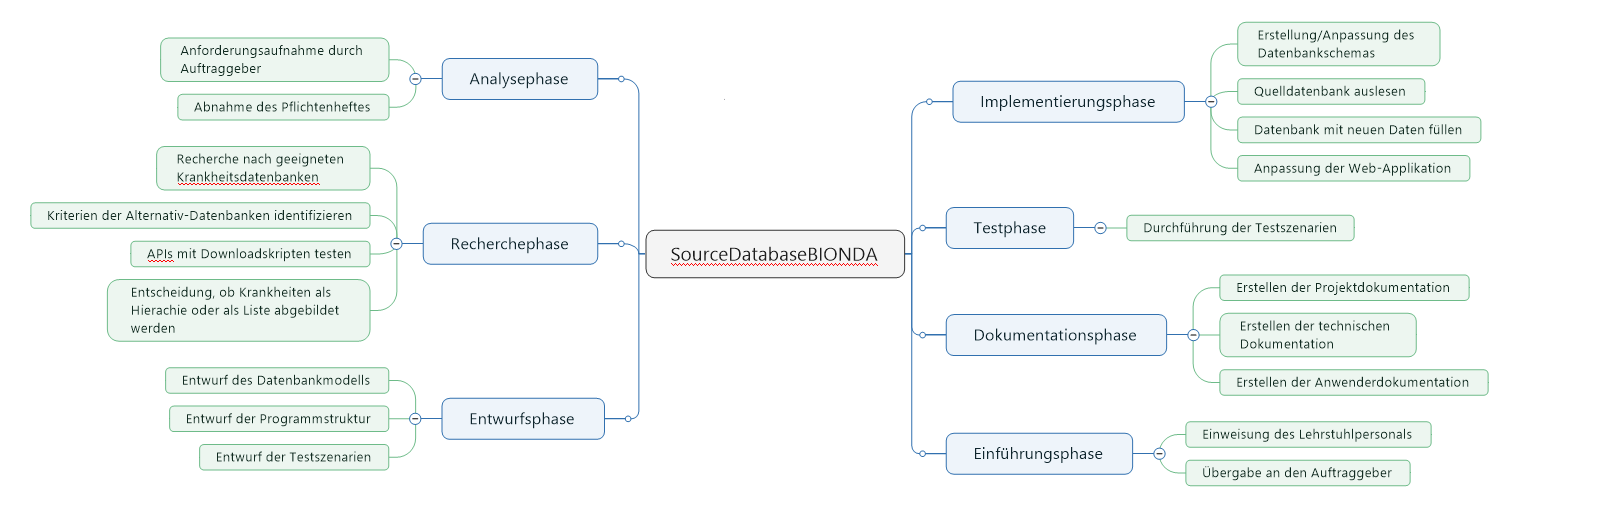
\includegraphics[scale=0.385]{bilder/Projektuebersicht.png}
\caption*{Projektphasen im Überblick}
\end{figure}

\begin{enumerate}
\item Analysephase
\begin{enumerate}[label*=\arabic*.]      
{\item Anforderungsaufnahme durch Auftraggeber} 
{\item Erstellung und Abnahme des Pflichtenheftes} 
\end{enumerate}
\item Recherchephase
\begin{enumerate}[label*=\arabic*.]
{\item Recherche nach geeigneten Krankheitsdatenbanken}       
{\item Kriterien der Alternativ-Datenbanken identifizieren} 
{\item APIs mit Downloadskripten testen} 
{\item Entscheidung, ob Krankheiten als Hierarchie oder als Liste abgebildet werden}
\end{enumerate}
\item Entwurfsphase
\begin{enumerate}[label*=\arabic*.]
{\item Entwurf des Datenbankmodells}       
{\item Entwurf der Programmstruktur} 
{\item Entwurf der Testszenarien} 
\end{enumerate}
\item Implementierungsphase
\begin{enumerate}[label*=\arabic*.]
{\item Erstellung/Anpassung des Datenbankschemas}       
{\item Quelldatenbank auslesen} 
{\item Datenbank mit neuen Daten füllen} 
{\item Anpassung der Web-Applikation}
\end{enumerate}
\item Testphase
\begin{enumerate}[label*=\arabic*.]  
{\item Durchführung der Testszenarien} 
\end{enumerate}
\item Dokumentationsphase
\begin{enumerate}[label*=\arabic*.]
{\item Erstellen der Projektdokumentation}       
{\item Erstellen der technischen Dokumentation}  
{\item Erstellen der Anwenderdokumentation} 
\end{enumerate}
\item Einführungsphase
\begin{enumerate}[label*=\arabic*.]
{\item Einweisung des Lehrstuhlpersonals}       
{\item Übergabe an den Auftraggeber} 
\end{enumerate}
\end{enumerate}

\section*{Arbeitspakete}
Jede Phase des Projekts wurde auch als Arbeitspaket zusammengefasst. Ein Arbeitspaket besteht aus Startdatum und Enddatum, sowie dem Name des Teammitgliedes, das für das Arbeitspaket zuständig ist. 

\subsection*{Analysephase}
\subsubsection*{Arbeitspaket 1.1: Anforderungsaufnahme durch Auftraggeber}
\begin{itemize}
\item Startdatum: 07.10.19
\item Enddatum: 29.10.19
\item Voraussetzung: -
\item Ergebnis: Anforderungen an die Software
\item Verantwortung: Projektteam
\end{itemize}
\subsubsection*{Arbeitspaket 1.2: Erstellung und Abnahme des Pflichtenheftes}
\begin{itemize}
\item Startdatum: 07.10.19
\item Enddatum: 29.10.19
\item Voraussetzung: -
\item Ergebnis: Pflichtenheft
\item Verantwortung: Projektteam
\end{itemize}
\subsection*{Recherchephase}
\subsubsection*{Arbeitspaket 2.1: Recherche nach geeigneten Krankheitsdatenbanken}
\begin{itemize}
\item Startdatum: 19.10.19
\item Enddatum: 25.10.19
\item Voraussetzung: -
\item Ergebnis: Krankheitsdatenbank-Kandidaten liegen vor
\item Verantwortung: Projektteam
\end{itemize}

\subsubsection*{Arbeitspaket 2.2: Kriterien der Alternativ-Datenbanken identifizieren}
\begin{itemize}
\item Startdatum: 19.10.19
\item Enddatum: 25.10.19
\item Voraussetzung: -
\item Ergebnis: Kriterien für den Vergleich liegen vor 
\item Verantwortung: Projektteam
\end{itemize}
\subsubsection*{Arbeitspaket 2.3: APIs mit Download-Skripten testen}
\begin{itemize}
\item Startdatum: 30.10.19
\item Enddatum: 08.11.19
\item Voraussetzung: AP 2.1
\item Ergebnis: Alternativ-DB für BIONDA
\item Verantwortung: Projektteam
\end{itemize}
\subsubsection*{Arbeitspaket 2.4: Entscheidung, ob Krankheiten als Hierarchie oder als Liste abgebildet werden}
\begin{itemize}
\item Startdatum:08.11.19
\item Enddatum: 17.11.19
\item Voraussetzung: AP 2.1, AP 2.3
\item Ergebnis: Plan für die Entwurfsphase
\item Verantwortung: Projektteam
\end{itemize}
\subsection*{Entwurfsphase}
\subsubsection*{Arbeitspaket 3.1: Entwurf des Datenbankmodells}
\begin{itemize}
\item Startdatum: 18.11.19
\item Enddatum: 24.11.19
\item Voraussetzung: AP 2.4
\item Ergebnis: Datenbankmodell
\item Verantwortung: P1
\end{itemize}

\subsubsection*{Arbeitspaket 3.2: Entwurf der Programmstruktur}
\begin{itemize}
\item Startdatum: 18.11.19
\item Enddatum: 24.11.19
\item Voraussetzung: AP 2.4
\item Ergebnis: Programmstruktur
\item Verantwortung: P2
\end{itemize}
\subsubsection*{Arbeitspaket 3.3: Entwurf der Testszenarien}
\begin{itemize}
\item Startdatum: 18.11.19
\item Enddatum: 24.11.19
\item Voraussetzung: AP 2.4
\item Ergebnis: Testszenarien
\item Verantwortung: P3
\end{itemize}
\subsection*{Implementierungsphase}
\subsubsection*{Arbeitspaket 4.1: Erstellung/Anpassung des Datenbankschemas}
\begin{itemize}
\item Startdatum: 25.11.19
\item Enddatum: 09.12.19
\item Voraussetzung: AP 2.1-2.4, AP 3.1-3.3
\item Ergebnis: Angepasstes Datenbankschema
\item Verantwortung: Projektteam
\end{itemize}
\subsubsection*{Arbeitspaket 4.2: Quelldatenbank auslesen}
\begin{itemize}
\item Startdatum: 25.11.19
\item Enddatum: 09.12.19
\item Voraussetzung: AP 2.1-2.4, AP 3.1-3.3
\item Ergebnis: Geparste Dateien
\item Verantwortung: Projektteam
\end{itemize}
\subsubsection*{Arbeitspaket 4.3: Datenbank mit neuen Daten füllen}
\begin{itemize}
\item Startdatum: 09.12.20
\item Enddatum: 19.12.20
\item Voraussetzung: AP 4.1
\item Ergebnis: Integration der Alternativ-Datenbank
\item Verantwortung: Projektteam
\end{itemize}
\subsubsection*{Arbeitspaket 4.4: Anpassung der Web-Applikation}
\begin{itemize}
\item Startdatum: 06.01.20
\item Enddatum: 10.01.20
\item Voraussetzung: AP 4.3
\item Ergebnis: Angepasste Webseite
\item Verantwortung: Projektteam
\end{itemize}
\subsection*{Testphase}
\subsubsection*{Arbeitspaket 5.1: Durchführung der Testszenarien}
\begin{itemize}
\item Startdatum: 11.01.20
\item Enddatum: 11.01.20
\item Voraussetzung: Testszenarien
\item Ergebnis: Es ist bekannt, ob die Software alle Tests erfolgreich durchläuft
\item Verantwortung: Projektteam
\end{itemize}
\subsection*{Dokumentationsphase}
\subsubsection*{Arbeitspaket 6.1: Erstellen der Projektdokumentation}
\begin{itemize}
\item Startdatum: 12.01.20
\item Enddatum: 24.01.20
\item Voraussetzung: fertige Software
\item Ergebnis: Dokumentation über das Projekt
\item Verantwortung: Projektteam
\end{itemize}
\subsubsection*{Arbeitspaket 6.2: Erstellen der technischen Dokumentation}
\begin{itemize}
\item Startdatum: 12.01.20
\item Enddatum: 24.01.20
\item Voraussetzung: fertige Software
\item Ergebnis: Dokumentation über die technischen Hintergründe der Software
\item Verantwortung: Projektteam
\end{itemize}
\subsubsection*{Arbeitspaket 6.3: Erstellen der Anwenderdokumentation}
\begin{itemize}
\item Startdatum: 12.01.20
\item Enddatum: 24.01.20
\item Voraussetzung: fertige Software
\item Ergebnis: Dokumentation für den Anwender
\item Verantwortung: Projektteam
\end{itemize}
\subsubsection*{Arbeitspaket 6.4: Pufferzeit}
\begin{itemize}
\item Startdatum: 24.01.20
\item Enddatum: 31.01.20
\item Voraussetzung: unfertige Arbeitspakete
\item Ergebnis: Vollendung der fehlenden Arbeitspakete 
\item Verantwortung: Projektteam
\end{itemize}
\subsection*{Einführungsphase}
\subsubsection*{Arbeitspaket 7.1: Einweisung des Lehrstuhlpersonals}
\begin{itemize}
\item Startdatum: 02.02.20
\item Enddatum: 02.02.20
\item Voraussetzung: fertige Software
\item Ergebnis: Lehrstuhlpersonal ist in die Software eingewiesen
\item Verantwortung: Projektteam
\end{itemize}
\subsubsection*{Arbeitspaket 7.2: Übergabe an den Auftraggeber}
\begin{itemize}
\item Startdatum: 07.02.20
\item Enddatum: 07.02.20
\item Voraussetzung: fertige Software
\item Ergebnis: Software an den Lehrstuhl übergeben
\item Verantwortung: Projektteam
\end{itemize}

\section*{Meilensteine}
Jede Phase des Projekts endet mit einem Meilenstein. Beim Erreichen des Meilensteins besteht die Möglichkeit die beendete Phase zu überprüfen und einen dieser 3 Wege zu wählen: 

\begin{enumerate}
\item Alle bisherigen Aktivitäten befinden sich im Plan, die Phase kann abgeschlossen werden, das Projekt kann wie geplant fortgesetzt werden.
\item Einige Aktivitäten, die eigentlich laut Planung bereits abgeschlossen sein sollten, weisen in den relevanten Größen (Kosten, Termine, Ergebnisse) signifikante Abweichungen auf. Es muss nachgearbeitet werden, um die Phase abschließen zu können.
\item Es sind Ereignisse eingetreten, die eine sinnvolle Projektfortsetzung unmöglich erscheinen lassen, das Projekt wird gestoppt und ggfs. ganz eingestellt oder unter neuen Rahmenbedingungen völlig neu aufgestellt.
\end{enumerate}

Des Weiteren wird jeder Meilenstein eine Anzahl von Arbeitspaketen zugewiesen. Diese Arbeitspakete sollten zur Deadline des Meilensteins erreicht sein, um eine Verzögerung des Projekts zu vermeiden. Nachfolgend werden die Meilensteine (MS) und Arbeitspakete aufgelistet:

\subsection*{MS 1: Analysephase beendet}
\subsubsection*{Deadline: 29.10.19}
\begin{itemize}
\item Arbeitspaket 1.1: Anforderungsaufnahme durch Auftraggeber
\item Arbeitspaket 1.2: Erstellung und Abnahme des Pflichtenheftes
\end{itemize}

\subsection*{MS 2: Recherchephase beendet}
\subsubsection*{Deadline: 17.11.19}
\begin{itemize}
\item Arbeitspaket 2.1: Recherche nach geeigneten Krankheitsdatenbanken
\item Arbeitspaket 2.2: Kriterien der Alternativ-Datenbank identifizieren
\item Arbeitspaket 2.3: APIs mit Download-Skripten testen
\item Arbeitsoaket 2.4: Entscheidung, ob Krankenheiten als Hierarchie oder Liste abgebildet werden
\end{itemize}

\subsection*{MS 3: Entwurfsphase beendet}
\subsubsection*{Deadline: 24.11.19}
\begin{itemize}
\item Arbeitspaket 3.1: Entwurf des Datenbankmodells
\item Arbeitspaket 3.2: Entwurf der Programmstruktur
\item Arbeitspaket 3.3: Entwurf der Testszenarien
\end{itemize}


\subsection*{MS 4: Implementierungsphase beendet}
\subsubsection*{Deadline: 10.01.20}
\begin{itemize}
\item Arbeitspaket 4.1: Erstellung/Anpassung des Datenbankschemas
\item Arbeitspaket 4.1: Quelldatenbank auslesen
\item Arbeitspaket 4.2: Datenbank mit neuen Daten füllen
\item Arbeitspaket 4.3: Anpassung der Web-Applikation
\end{itemize}

\subsection*{MS 5: Testphase beendet}
\subsubsection*{Deadline: 11.01.20}
\begin{itemize}
\item Arbeitspaket 5.1: Durchführung der Testszenarien
\end{itemize}

\subsection*{MS 6: Dokumentationsphase beendet}
\subsubsection*{Deadline: 24.01.20}
\begin{itemize}
\item Arbeitspaket 6.1: Erstellen der Projektdokumentation
\item Arbeitspaket 6.2: Erstellen der technischen Dokumentation
\item Arbeitspaket 6.3: Erstellen der Anwenderdokumentation
\end{itemize}

\subsection*{MS 7: Pufferzeit ausgeschöpft}
\subsubsection*{Deadline: 31.01.20}
\begin{itemize}
\item Arbeitspaket 6.4: Pufferzeit
\end{itemize}

\subsection*{MS 8: Projekt abgeschlossen}
\subsubsection*{Deadline: 07.02.20}
\begin{itemize}
\item Arbeitspaket 7.1: Einweisung des Lehrstuhlpersonals
\item Arbeitspaket 7.2: Übergabe an den Auftraggeber
\end{itemize}

\begin{figure}[h]
\centering
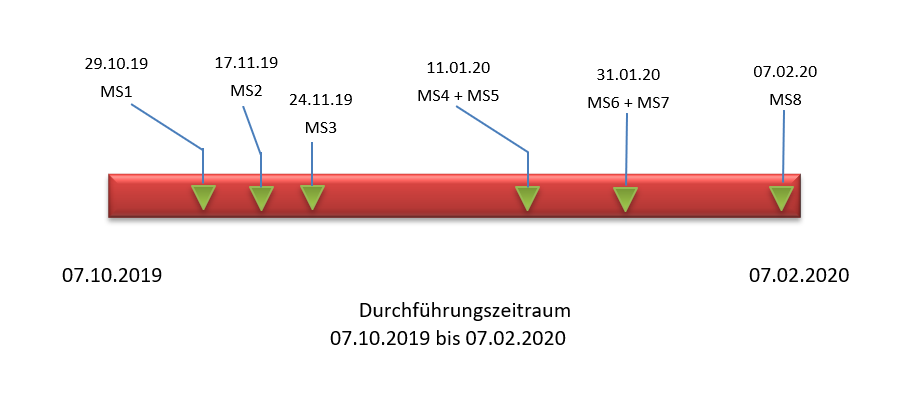
\includegraphics[scale=1]{bilder/Meilensteinplan.png}
\caption*{Meilensteine im Überblick}
\end{figure}
\chapter*{Qualitätsanforderung}
Im Folgenden werden die wesentlichen Qualitätsanforderungen erläutert.

\section*{Erweiterbarkeit}
Die zu entwickelnde Softwarestruktur muss so gewählt werden, dass eine einfache Implementierung der angedachten Erweiterungen möglich ist. 
Mögliche Erweiterungen oder Änderungen bereits implementierter Funktionen sollen mit geringem zeitlichem Aufwand durchgeführt werden können, ohne dass eine tief greifende Umstrukturierung des bestehenden Quellcodes vorgenommen werden muss. 

\section*{Fehlerrobustheit}
Alle während des Betriebes auftretende Fehler und Warnungen müssen abgefangen und zur Anzeige gebracht werden. Im Fehlerfall muss der laufende Prozess kontrolliert abgebrochen werden. Zusätzlich muss entschieden werden, ob die Schwere des Fehlers einen Programmabbruch zur Folge haben soll. Angefallene Fehler sollen in einer lokal gespeicherten Datei protokolliert werden. 

\section*{Wartbarkeit}
Um eine langfristige Nutzung der Software zu ermöglichen, muss das Projekt so aufgebaut und dokumentiert sein, dass die Administration, Wartung und Weiterentwicklung ohne großen Einarbeitungsaufwand von einem anderen Entwickler oder Administrator durchgeführt werden kann. 
Um dies zu gewährleisten, muss die Anwendung modular programmiert und exakt dokumentiert sein. 
Dazu gehören eine Projektdokumentation, eine Anwenderdokumentation und eine technische Dokumentation. 
\chapter*{Testszenarien}
Die folgenden Tabellen stellen die Testfälle dar, die sich aus den Qualitätsanforderungen ableiten. Diese müssen nach der Implementierung des Projektes durchgeführt und erfolgreich durchlaufen werden. Jedes der folgenden Testszenarien muss auf allen unter Punkt 5.3 genannten Client-Betriebssystemen und Server-Betriebssystemen mit dem Ergebnis „bestanden“ durchlaufen werden.

\section*{QS-Ziele}

\begin{table}[!htbp]
\centering
\label{my-label}
\begin{tabular}{|l|l|l|}
\hline
\rowcolor[HTML]{EFEFEF} 
\multicolumn{1}{|c|}{\cellcolor[HTML]{EFEFEF}{\color[HTML]{333333} QS-Ziel}} & \multicolumn{1}{c|}{\cellcolor[HTML]{EFEFEF}{\color[HTML]{333333} Prüfung}} & \multicolumn{1}{c|}{\cellcolor[HTML]{EFEFEF}{\color[HTML]{333333} Bestanden}} \\ \hline
Erweiterbarkeit                                                              & Integrierung von weiteren Funktionen                                        &                                                                               \\ \hline
Fehlerrobustheit                                                             & s. Punkt 5.2                                                                &                                                                               \\ \hline
Wartbarkeit                                                                  & Test durch zweiten Entwickler                                               &                                                                               \\ \hline
\end{tabular}
\caption*{QS-Ziele}
\end{table}

Des Weiteren muss eine Auswahl einer neuen alternativen Datenbank erfolgen. Da es sehr viele mögliche Datenbanken gibt, die der Aufgabenstellung entsprechen,  muss eine Entscheidung anhand von verschiedenen Kriterien getroffen werden. Die folgende Tabelle stellt fünf Kriterien dar, welche bei der Wahl der neuen alternativen Datenbank berücksichtigt werden müssen. Um eine Entscheidung treffen zu können müssen die verschiedenen Kriterien gewichtet werden, um besser abwägen zu können, welche der Möglichkeiten die bestmögliche ist. Die Gewichtung der verschiedenen Kriterien ist ebenfalls in der Tabelle abgebildet.
 
\begin{table}[!htbp]
\centering
\label{my-label}
\begin{tabular}{|l|l|l|}
\hline
\rowcolor[HTML]{EFEFEF} 
\multicolumn{1}{|c|}{\cellcolor[HTML]{EFEFEF}{\color[HTML]{333333} Kriterium}} & \multicolumn{1}{c|}{\cellcolor[HTML]{EFEFEF}{\color[HTML]{333333} Faktor}} & \multicolumn{1}{c|}{\cellcolor[HTML]{EFEFEF}{\color[HTML]{333333} Rang}} \\ \hline
Updatehäufigkeit & $\times 2$                                        &                       4                                                        \\ \hline
Anzahl an Einträgen                                                             &                                                                $\times 5$ &        1                                                                       \\ \hline
Kostenlos und frei zugänglich                                                                  & $\times 3$                                              &                                                                              3 \\ \hline
Von öffentlicher Organisation
& $\times 4$                                                               &                                                                              2 \\ \hline
Suche anhand Trivialnamen
& $\times 1$                                                               &                                                                              5 \\ \hline
\end{tabular}
\caption*{Kriterien der Quelldatenbank}
\end{table}

\newpage
\section*{Fehlerrobustheit}

Testszenarien können in den verschiedenen Projektphasen ermittelt bzw. erstellt werden. Die wichtigeten Testszenarien sind jedoch die, die am Ende für den Test der neu angebundenen Datenbank erfolgen. Durch diese wird sichergestellt, dass BIONDA durch die neu angebundene Datenbank dazu in der Lage ist, deutlich mehr Suchtreffer für diverse Krankheiten zu liefern.

\begin{table}[h]
\begin{tabular}{|c|c|c|}
\hline
\textbf{Fehler}                                                                                                                    & \textbf{Erwartete Reaktion}                                                                        & \textbf{Bestanden} \\ \hline
\begin{tabular}[c]{@{}c@{}}Suche nach Krankheit mithilfe eines \\ Unterbegriffs zeigt nicht \\ korrekte Hierarchie an\end{tabular} & \begin{tabular}[c]{@{}c@{}}Gesamthierarchie anzeigen, \\ Fehler protokolliere\end{tabular}         &                    \\ \hline
\begin{tabular}[c]{@{}c@{}}Suche nach Krankheit mithilfe des\\ Oberbegriffs zeigt nicht \\ korrekte Hierarchie an\end{tabular}     & \begin{tabular}[c]{@{}c@{}}Gesamthierarchie anzeigen, \\ Fehler protokollieren\end{tabular}        &                    \\ \hline
\begin{tabular}[c]{@{}c@{}}Suche nach Biomarker, welcher einer \\ Krankheit gehört, \\ gibt falsche Krankheit an\end{tabular}      & \begin{tabular}[c]{@{}c@{}}Alternative Krankheiten anzeigen, \\ Fehler protokollieren\end{tabular} &                    \\ \hline
\begin{tabular}[c]{@{}c@{}}Downloadskript konnte Quelldatenbank \\ nicht ansprechen\end{tabular}                                   & \begin{tabular}[c]{@{}c@{}}Fehler protokollieren, \\ Wiederholung in einer Stunde\end{tabular}     &                    \\ \hline
\end{tabular}
\caption*{Fehlerrobustheit}
\end{table}
\chapter*{Produktumgebung}


\section*{Anforderungen an die Produktumgebung}
Für das Produkt wird ein Linuxserver benötigt, um die Webapplikation \enquote{BIONDA} bereitzustellen. Des Weiteren wird ein MySQL-Server benötigt, um alle nötigen Informationen für \enquote{BIONDA} zu speichern. Beides wird vom Auftraggeber bereitgestellt. 


\section*{Anforderungen an die Entwicklungsumgebung}
Hinsichtlich der Auswahl der zu benutzenden Entwicklungsumgebung gibt es keine Einschränkungen. Es muss aber gewährleistet sein, dass sämtliche Anforderungen erfüllt werden können. Insbesondere muss die Ausführung von Python, Java und Perl Programmen möglich sein. Des Weiteren wird vom Auftraggeber eine Testinfrastruktur zur Verfügung gestellt, um die nötigen Entwicklungsschritte zu testen. 


\chapter{Activity Diagram of Application}
\label{Anhang_AktivDiaRUBBauteilerkennung}
\begin{figure}[H]
\centering
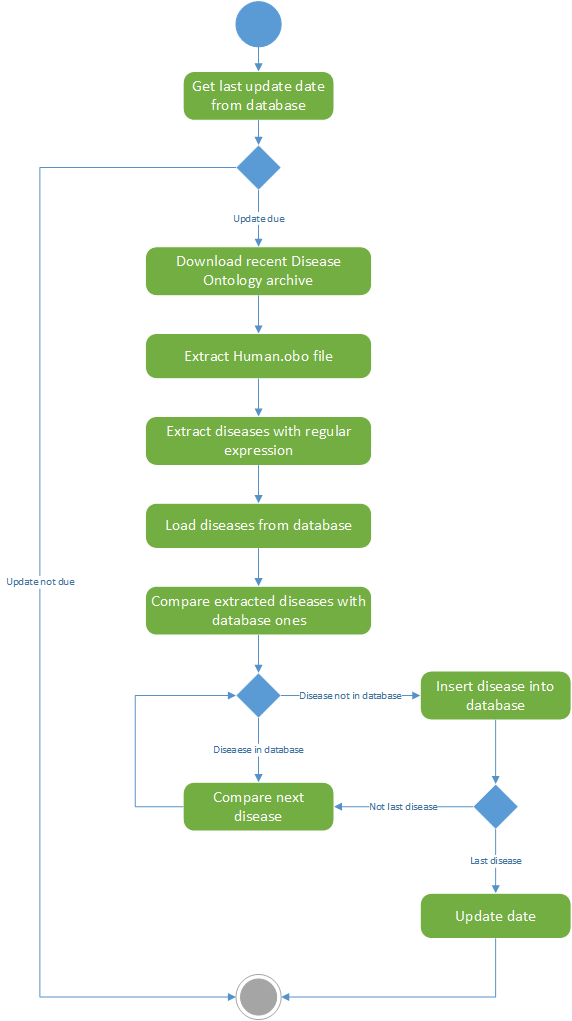
\includegraphics[scale=0.75]{bilder/Aktivitaetsdiagramm_Grundliegenderablauf.png}
\caption{Activity Diagram of Application}
\end{figure}

\chapter{Entity Relationship Model}
\label{Anhang_ER}
\vspace*{\fill}
\begin{figure}[H]
\centering
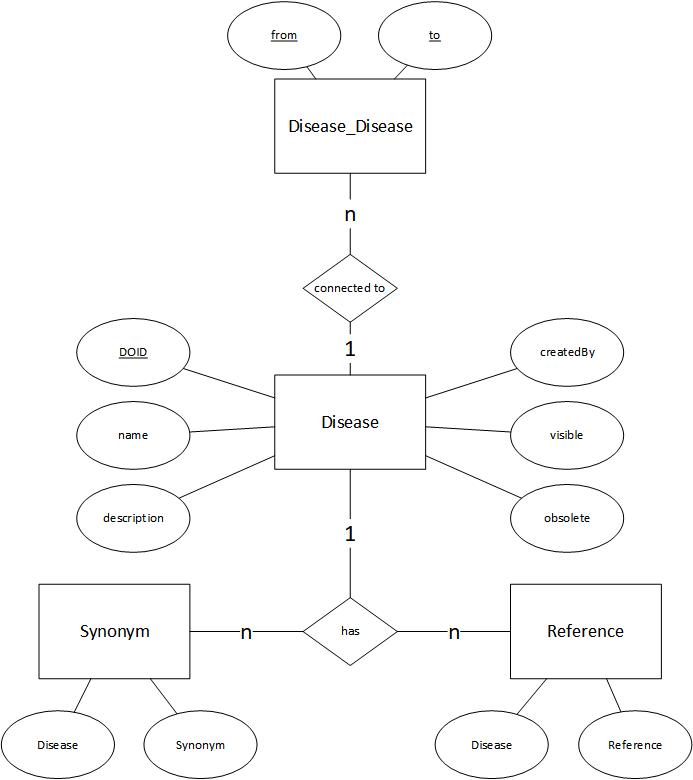
\includegraphics[scale=0.75]{bilder/ER.png}
\caption{Entity Relationship Model}
\end{figure}
\vspace*{\fill}

\chapter{Database Schema}
\label{Anhang_UMLDatenbankschema}
\begin{figure}[H]
\centering
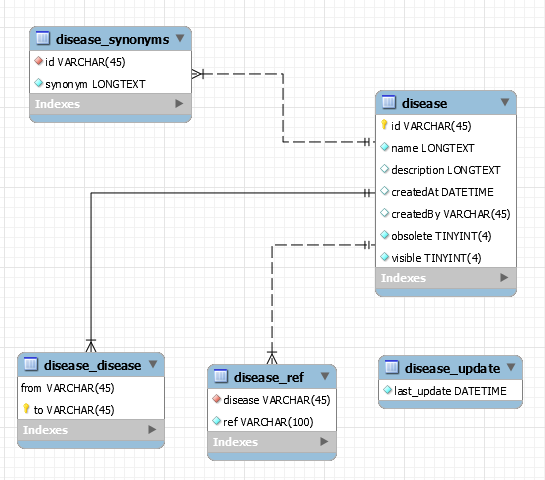
\includegraphics[scale=1]{bilder/db_schema.png}
\caption{Database Schema Modifications}
\end{figure}
\section*{SQL-Statements}
Following are the SQL statements that are necessary for adding and modify the current database of Bionda.\\

\begin{lstlisting}[
           language=sql,
           showspaces=false,
           basicstyle=\ttfamily,
           numbers=left,
           numberstyle=\tiny,
           commentstyle=\color{gray}
        ]
--
-- Table structure for table `disease`
--

DROP TABLE IF EXISTS `disease`;
CREATE TABLE `disease` (
  `id` varchar(45) NOT NULL,
  `name` longtext CHARACTER SET utf8mb4 
  COLLATE utf8mb4_0900_ai_ci NOT NULL,
  `description` longtext CHARACTER SET utf8mb4 
  COLLATE utf8mb4_0900_ai_ci,
  `createdAt` datetime DEFAULT NULL,
  `createdBy` varchar(45) CHARACTER SET latin1 
  COLLATE latin1_swedish_ci DEFAULT NULL,
  `obsolete` tinyint(4) NOT NULL DEFAULT '0',
  `visible` tinyint(4) NOT NULL DEFAULT '1',
  PRIMARY KEY (`id`)
) ENGINE=InnoDB DEFAULT CHARSET=utf8mb4 
COLLATE=utf8mb4_0900_ai_ci;

--
-- Table structure for table `disease_disease`
--

DROP TABLE IF EXISTS `disease_disease`;
CREATE TABLE `disease_disease` (
  `from` varchar(45) NOT NULL,
  `to` varchar(45) NOT NULL,
  PRIMARY KEY (`from`,`to`),
  CONSTRAINT `from` FOREIGN KEY (`from`) 
  REFERENCES `disease` (`id`) 
  ON DELETE CASCADE ON UPDATE CASCADE
) ENGINE=InnoDB DEFAULT CHARSET=utf8mb4 
COLLATE=utf8mb4_0900_ai_ci;

--
-- Table structure for table `disease_ref`
--

DROP TABLE IF EXISTS `disease_ref`;
CREATE TABLE `disease_ref` (
  `disease` varchar(45) NOT NULL,
  `ref` varchar(100) NOT NULL,
  KEY `disease_idx` (`disease`),
  CONSTRAINT `disease` FOREIGN KEY (`disease`) 
  REFERENCES `disease` (`id`) 
  ON DELETE CASCADE ON UPDATE CASCADE
) ENGINE=InnoDB DEFAULT CHARSET=utf8mb4 
COLLATE=utf8mb4_0900_ai_ci;

--
-- Table structure for table `disease_synonyms`
--

DROP TABLE IF EXISTS `disease_synonyms`;
CREATE TABLE `disease_synonyms` (
  `id` varchar(45) NOT NULL,
  `synonym` longtext NOT NULL,
  KEY `disease_idx` (`id`),
  KEY `disease_syn_idx` (`id`),
  CONSTRAINT `disease_syn` FOREIGN KEY (`id`) 
  REFERENCES `disease` (`id`) 
  ON DELETE CASCADE ON UPDATE CASCADE
) ENGINE=InnoDB DEFAULT CHARSET=utf8mb4 
COLLATE=utf8mb4_0900_ai_ci;

--
-- Table structure for table `disease_update`
--

DROP TABLE IF EXISTS `disease_update`;
CREATE TABLE `disease_update` (
  `last_update` datetime NOT NULL
) ENGINE=InnoDB DEFAULT CHARSET=utf8mb4 
COLLATE=utf8mb4_0900_ai_ci;
\end{lstlisting}

\chapter{Class Diagram}
\label{Anhang_Klassendiagramm}
\vspace*{\fill}
\begin{figure}[H]
\centering
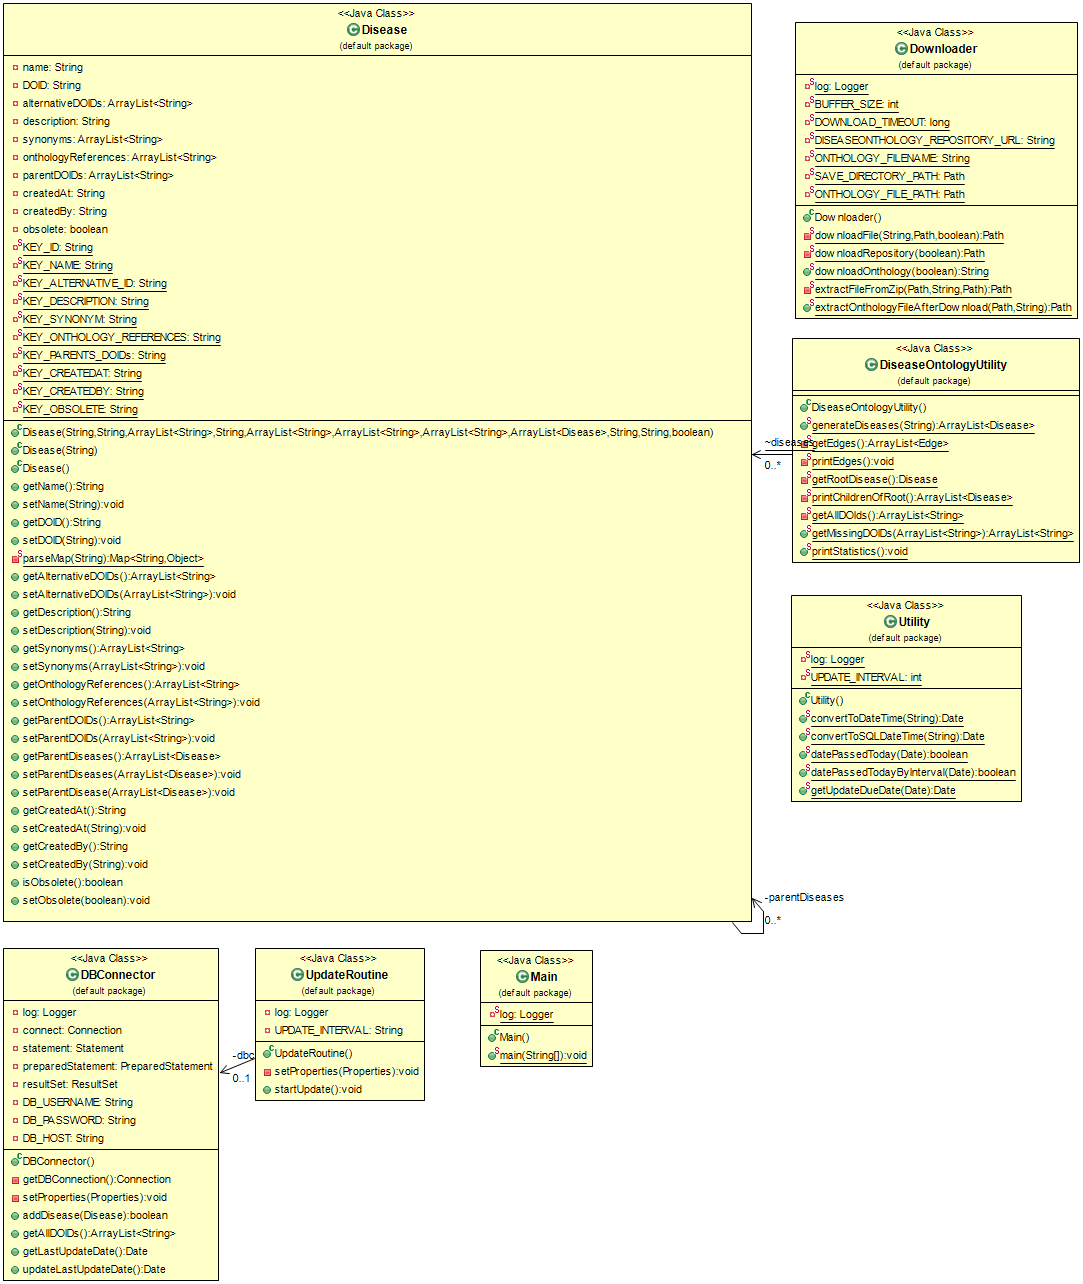
\includegraphics[scale=0.4]{bilder/UpdateDatabaseClassDiagram.png}
\caption{Class Diagram of Application}
\end{figure}
\vspace*{\fill}

\chapter{Snippet of Diseases in HumanDO.obo}
\label{Anhang_SnippetDiseases}
\begin{figure}[H]
\centering
\begin{lstlisting}[]
[Term]
id: DOID:0001816
name: angiosarcoma
alt_id: DOID:267
alt_id: DOID:4508
def: "A vascular cancer that derives from the cells that line the walls of blood vessels or
lymphatic vessels." [url:http\://emedicine.medscape.com/article/276512-overview, 
url:http\://en.wikipedia.org/wiki/Hemangiosarcoma, 
url:https\://en.wikipedia.org/wiki/Angiosarcoma, 
url:https\://www.ncbi.nlm.nih.gov/pubmed/23327728]
subset: NCIthesaurus
synonym: "hemangiosarcoma" EXACT []
xref: MESH:D006394
xref: NCI:C3088
xref: NCI:C9275
xref: SNOMEDCT_US_2018_03_01:33176006
xref: SNOMEDCT_US_2018_03_01:39000009
xref: UMLS_CUI:C0018923
xref: UMLS_CUI:C0854893
is_a: DOID:175 ! vascular cancer

[Term]
id: DOID:0002116
name: pterygium
def: "A corneal disease that is characterized by a triangular tissue growth located_in cornea
of the eye that is the result of collagen degeneration and fibrovascular proliferation."
[url:https\://en.wikipedia.org/wiki/Pterygium_(conjunctiva)]
synonym: "surfer's eye" EXACT []
xref: MESH:D011625
xref: UMLS_CUI:C0033999
is_a: DOID:10124 ! corneal disease
created_by: laronhughes
creation_date: 2010-06-30T02:44:30Z

[Term]
id: DOID:0014667
name: disease of metabolism
def: "A disease that involving errors in metabolic processes of building or degradation of
molecules." [url:http\://www.ncbi.nlm.nih.gov/books/NBK22259/]
subset: DO_AGR_slim
subset: NCIthesaurus
synonym: "metabolic disease" EXACT [SNOMEDCT_2005_07_31:75934005]
xref: ICD10CM:E88.9
xref: ICD9CM:277.9
xref: MESH:D008659
xref: NCI:C3235
xref: SNOMEDCT_US_2018_03_01:30390004
xref: SNOMEDCT_US_2018_03_01:75934005
xref: UMLS_CUI:C0025517
is_a: DOID:4 ! disease
\end{lstlisting}
\caption{Snippet of Diseases in Human.obo File}
Source: \citep{do}
\end{figure}


\chapter{Example of Pattern Matching of Diseases}
\label{Anhang_PatterMatching}
\begin{figure}[H]
\centering
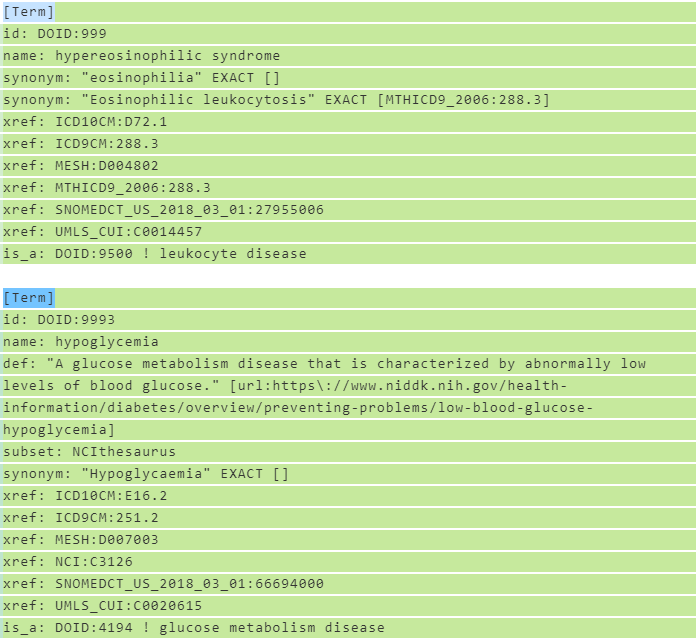
\includegraphics[scale=0.68]{bilder/regex_match1.png}
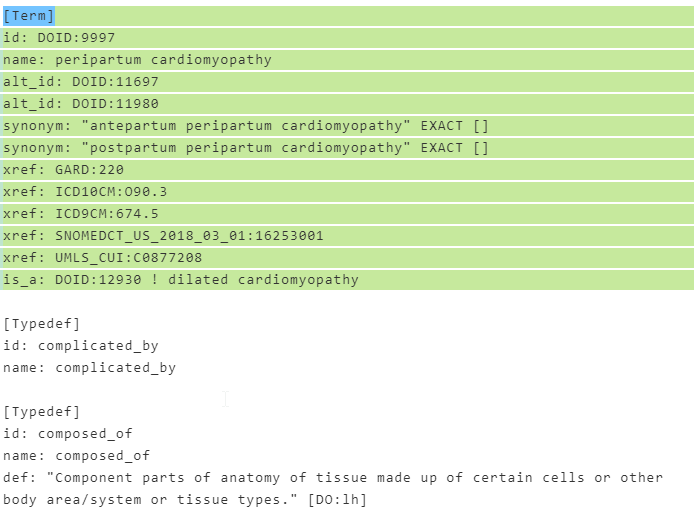
\includegraphics[scale=0.68]{bilder/regex_match2.png}
\caption{Example Pattern Matching of Diseases}
(Green: Group Match, Blue+Green: Full Match)
\end{figure}

\chapter{Error List}
\label{Anhang_ErrorList}

\begin{table}[H]
\resizebox{\textwidth}{!}{%
\begin{tabular}{|l|l|l|}
\hline
\textbf{Error Code} & \textbf{Error}                                                                                                                                             & \textbf{Class}                                                                             \\ \hline
100                 & Couldn't read Application Properties                                                                                                                       & \begin{tabular}[c]{@{}l@{}}Downloader, UpdateRoutine, \\ DBConnector, Utility\end{tabular} \\ \hline
110                 & Couldn't set Application Properties                                                                                                                        & \begin{tabular}[c]{@{}l@{}}Downloader, UpdateRoutine, \\ DBConnector, Utility\end{tabular} \\ \hline
120                 & \begin{tabular}[c]{@{}l@{}}Couldn't set update interval. Wrong number? \\ Please set a number as string\end{tabular}                                       & Utility                                                                                    \\ \hline
130                 & \begin{tabular}[c]{@{}l@{}}Couldn't set buffer\_size/timeout. \\ Wrong number/long? \\ Please set a number/long as string\end{tabular}                     & Downloader                                                                                 \\ \hline
200                 & \begin{tabular}[c]{@{}l@{}}Connection to the database \\ couldnt be established. Wrong credentials?\end{tabular}                                           & DBConnector                                                                                \\ \hline
210                 & \begin{tabular}[c]{@{}l@{}}Disease couldn't be inserted into the \\ database due to an SQL Error\end{tabular}                                              & DBConnector                                                                                \\ \hline
220                 & \begin{tabular}[c]{@{}l@{}}Disease couldn't be inserted into the \\ database due to a SQL Date Parse Error\end{tabular}                                    & DBConnector                                                                                \\ \hline
230                 & Diseases DO ID couldnt be fetched from database.                                                                                                           & DBConnector                                                                                \\ \hline
240                 & \begin{tabular}[c]{@{}l@{}}Update record couldnt be fetched. \\ Maybe no first default entry?\end{tabular}                                                 & DBConnector                                                                                \\ \hline
250                 & Last update date couldn't be updated!                                                                                                                      & DBConnector                                                                                \\ \hline
000                 & Database connection couldnt be closed!                                                                                                                     & DBConnector                                                                                \\ \hline
300                 & \begin{tabular}[c]{@{}l@{}}Couldn't read HumanDO.obo file. \\ Does it exist in the home directory?\end{tabular}                                            & DiseaseOntologyUtility                                                                     \\ \hline
310                 & \begin{tabular}[c]{@{}l@{}}Couldn't process HumanDO.obo file. \\ Did it changed its size (\textgreater 2GB)?\end{tabular}                                  & DiseaseOntologyUtility                                                                     \\ \hline
320                 & \begin{tabular}[c]{@{}l@{}}Couldn't process HumanDO.obo file. \\ Something is wrong with the format of \\ the file or the regular expression!\end{tabular} & DiseaseOntologyUtility                                                                     \\ \hline
400                 & \begin{tabular}[c]{@{}l@{}}Couldn't compare update date with today. \\ Is update interval set right?\end{tabular}                                          & Main                                                                                       \\ \hline
410                 & \begin{tabular}[c]{@{}l@{}}Couldn't download DO archive. \\ Check stack trace for reason.\end{tabular}                                                     & Main                                                                                       \\ \hline
420                 & \begin{tabular}[c]{@{}l@{}}Something interrupted the download process. \\ Check stack trace for reason.\end{tabular}                                       & Main                                                                                       \\ \hline
010                 & \begin{tabular}[c]{@{}l@{}}Unexpected error occurred. \\ Check stack trace for reason.\end{tabular}                                                        & Main                                                                                       \\ \hline
\end{tabular}%
}
\caption{Documentation of Errors}
\label{tab:errorlist}
\end{table}

% dont remove
\addtocontents{toc}{\protect\setcounter{tocdepth}{1}}
